\section{Experiments}
\label{sec:results}
To test the proposed method, we conducted two different experiments. In the first experiment, we set up a controlled environment with heart and haze phantoms (\emph{in-vitro}). In the second experiment, we use hazy \emph{in-vivo} cardiac ultrasound data. All experimental data is recorded using an X5-1C matrix phased array transducer connected to a Philips EPIQ scanner (Philips Research, North America). The transducer has a frequency range of \qtyrange{1}{5}{\mega\hertz} and all acquisitions are made using harmonic imaging.
 
Even though the proposed dehazing method operates in the RF domain, all metrics (see sections \ref{sec:invitro}, \ref{sec:invivo}) are computed after log-compression and envelope-detection (B-mode), since the images are eventually displayed in that format. Lastly, all images are brightness matched by matching the average intensity of the top 10\% pixel values and plotted in the same dynamic range of \qty{60}{dB} for a fair visual comparison. 

\begin{figure*}
    \centering
    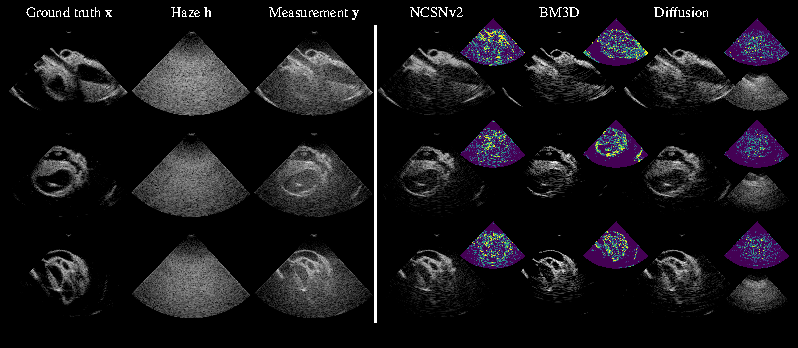
\includegraphics[width=\textwidth, clip, trim=0 0.3cm 0 0]{figures/steve7.pdf}
    \caption{\emph{In-vitro} results using the phantom data. The ground truth ultrasound $\bx$ and haze signals $\bh$ which are used to construct measurement $\by$ are shown on the left. RF-based dehazing results are on the right, for both the baseline methods (BM3D and NCSNv2) and the proposed diffusion method. For the latter, we show posterior solutions for both the ultrasound and haze signals (lower inset plot to the right). For all methods, we show error plots that highlight the difference between ground truth and dehazed images, with the proposed diffusion method notably dropping less signal.}
    \label{fig:comparison-invitro}    
\end{figure*}
\subsection{In-Vitro}
\label{sec:invitro}
To thoroughly examine the method's behavior, we conducted a controlled test using a heart phantom and a dedicated haze phantom (as described in Section~\ref{sec:haze_estimation}). This allowed us to collect two distinct sets of beamsummed RF data. These datasets were utilized to train the two diffusion models, $s_\theta$ and $s_\phi$, respectively. We acquired a total of $2\times150$ frames for the training dataset and $2\times38$ frames for validation, of both the heart and haze phantoms separately. During inference, we artificially add the haze signal to the heart phantom ultrasound data with \TSW{varying haze levels} to imitate the haze process and set the desired haze-to-signal ratio. This enables us to compare the dehazed output to the ground truth, ensuring that the extracted haze aligns with the desired haze distribution.
\vspace{-0.1cm}

\subsection{In-Vivo}
\label{sec:invivo}
In a second experiment, we train and deploy our method on an \emph{in-vivo} cardiac ultrasound dataset. In total, we acquired ultrasound data from five different human volunteers and used four different commonly used views to record the echocardiograms. Namely the apical three- and four-chamber view (AP3/AP4), parasternal long axis (PLAX), and short axis (PSAX) views. \TSW{Combined, the dataset comprises a total of 2640 frames collected from 6 volunteers. All 44 acquisitions consist of 60-frame sequences, each covering approximately a complete cardiac cycle. We divided this dataset into three main subsets: 1) a training set, earlier denoted as $\mathcal{X}$, consisting of 1500 clean frames from three volunteers which are used for training the tissue model, 2) a validation set comprising of 1020 frames from two other volunteers for validation of the proposed method, 3) another training set with the remaining 120 frames of the last volunteer. The latter two datasets are considered hazy and were acquired from technically difficult-to-image subjects. To generate the specialized haze-only training dataset $\mathcal{H}$ for training the haze model, we use the acquisitions from the third dataset combined with the relatively hazy parts of the first training dataset for augmentation. Subsequently, the generation of the haze-only images involves the apodization method outlined in Section~\ref{sec:haze_estimation}. This method extracts off-axis clutter by cancelation of the main lobes, effectively eliminating tissue signal and concentrating solely on haze characteristics. Lastly, as part of our methodology, we deliberately reserved 5 images from each of the tissue (1) and haze (3) training datasets. These images are exclusively used for fine-tuning both training and inference hyperparameters.}

\subsection{Metrics}
As a quantitative measure, we compute the peak signal-to-noise ratio (PSNR) between the dehazed output and ground truth images. The PSNR is a pixel-wise difference metric that normalizes the mean squared error between two images by the image range to account for different intensity ranges across examples. Unlike the \emph{in-vitro} experiment, there is no ground truth available for the \emph{in-vivo} data. Therefore, we compute the generalized contrast-to-noise ratio (gCNR) \cite{rodriguez-molaresGeneralizedContrasttonoiseRatio2020}, which is an unsupervised image quality metric, commonly used in ultrasound, given by:

\begin{equation}
    \mathrm{gCNR}(I) = 1 - \int_x \min\left\{ p_A(x), p_B(x) \right\} \mathrm{d}x,
\end{equation}
where $p_A$ and $p_B$ are the probability density functions for each of the regions of interest (ROIs). We compute a histogram for each ROI to estimate its distribution and choose the heart chamber (ventricle) near the apex (typically the most challenging and most hazy region) as region $A$ and part of the ventricular septum (wall) as region $B$. Most notably, the gCNR is not biased by dynamic range stretching and can thus provide a fair comparison independent of specific brightness settings. 

\TSW{To ensure accurate results, we manually draw two masks as ROIs for seven equidistant frames in each of the 60-frame sequences in the dataset, using a lasso selection tool. For the remaining frames, the masks are determined by linearly interpolating the vertices of a polygon, which are fitted to each mask using the Douglas-Peucker algorithm. This approach provides us with larger and more precise regions that move in} \TSW{synchronization with the cardiac cycle, as opposed to relying on a single set of ROIs per sequence. On average, the areas for regions $A$ and $B$ are \qty{14}{\cm\tothe{2}} and  \qty{8}{\cm\tothe{2}}, respectively}. We remove outliers by eliminating the scores below the $10$th percentile obtained from the measurement frames, as these frames are assumed to have inaccurate ROIs. Since we remove outliers based on scores from the raw harmonic data, this should not favor any of the proposed or baseline methods.

\TSW{Additionally, we utilize the Kolmogorov-Smirnov (KS) test to assess the ability of dehazing methods to retain speckle statistics in the myocardium regions. Furthermore, we investigate how the dehazing methods affect the ventricle region, which is expected to predominantly contain haze and no tissue signal. The KS statistic is defined as the greatest distance between the empirical distributions of two samples and serves as a measure of statistical similarity.} 

\TSW{Lastly, since the KS test only considers pixel statistics independently, we more closely investigate speckle characteristics, by estimating the speckle size. This provides us with a measure of the lateral resolution and insight into the spatial} \TSW{preservation of statistics. The speckle size is evaluated through measurement of the Full-Width at Half-Maxima (FWHM) of the lateral main lobe of the two-dimensional autocorrelation taken from the myocardium region in the polar domain. The same ROIs as for the gCNR computation are used for both the KS test and the FWHM estimation.}\color{black}

\begin{figure}
    \centering
    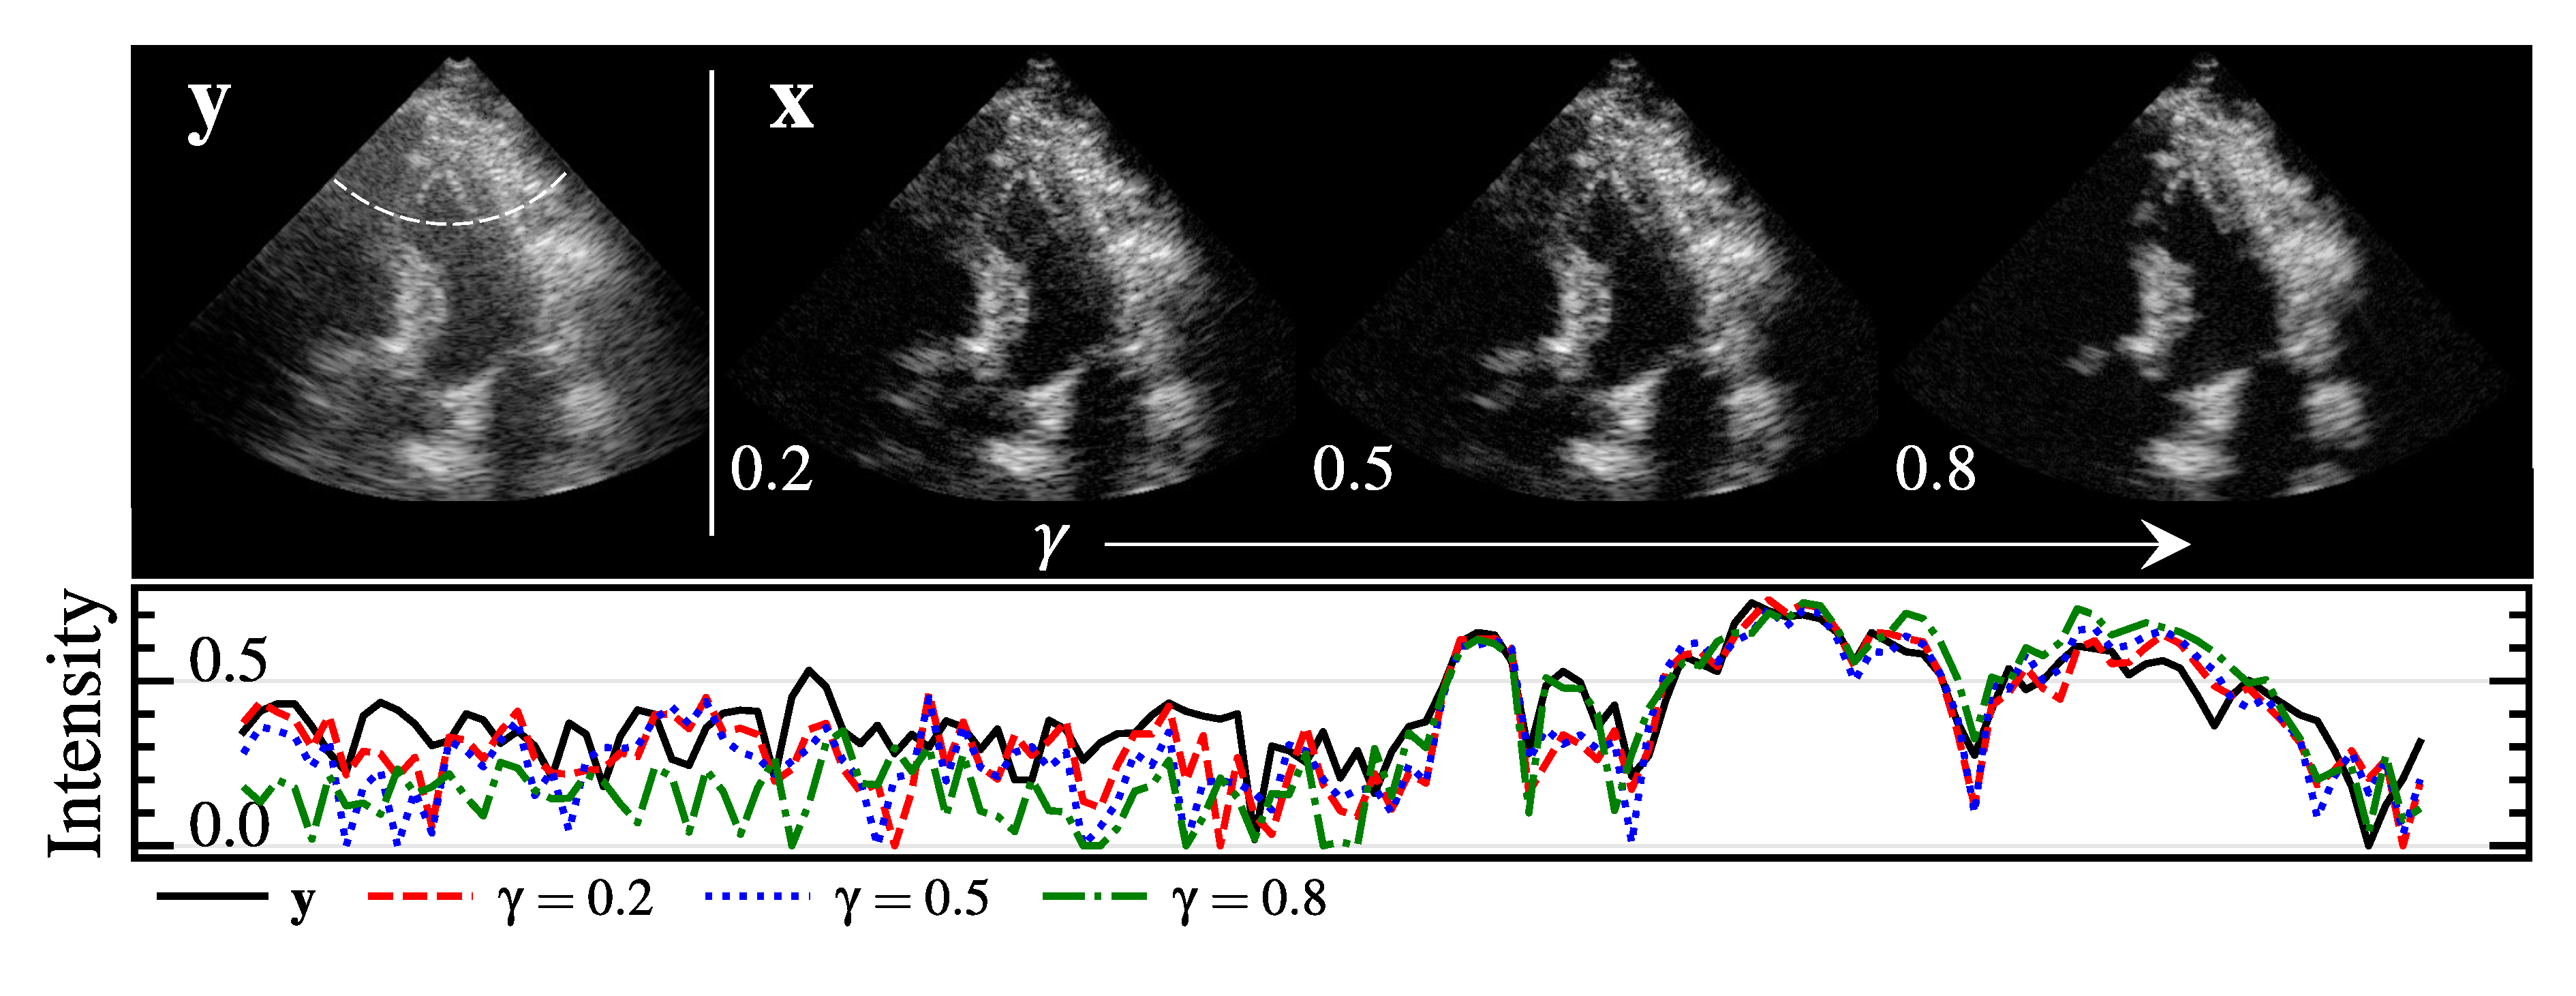
\includegraphics[scale=0.145, trim=2cm 3cm 0 0]{figures/steve8.pdf}
    \caption{Varying amount of dehazing using tunable haze amplitude parameter $\gamma$. A lateral cross-section is shown for a more detailed comparison. The exact slice is indicated by the white dashed line.}
    \label{fig:varying_gamma}
\end{figure}
\subsection{Baselines}
As a baseline method, we use the block-matching and 3D filtering algorithm (BM3D) \cite{dabovImageDenoisingBlockmatching2006}. BM3D has been a popular noise suppression algorithm and has recently been adopted for ultrasound \cite{santosUltrasoundImageDespeckling2017}. BM3D outperforms transform-based denoisers, which often fail to preserve details that are not represented in the 2D transform domain. Furthermore, BM3D is general concerning the type of noise. We adapted and fine-tuned BM3D for the cardiac dehazing problem to create a competitive baseline. To that end, we deploy BM3D in the RF domain, as the image domain results mainly introduce blurring of the images without any dehazing effect.

Additionally, we compare the proposed technique with a deep learning method. Specifically, we use a supervised deep learning approach, training the model end-to-end to tackle the dehazing task on a paired dataset. Although not readily available in the literature for dehazing, the U-Net has been the go-to neural architecture in medical image restoration. For a fair comparison, we use the same backbone network, NCSNv2, used in our diffusion approach, which is also a U-Net type network. We train the supervised network on the RF phantom dataset, as we only have pairs for this dataset. This is the inherently limiting part of the supervised approach.

\subsection{Downstream Delineation Task}
\label{sec:downstream}
\TSW{In the context of ultrasound imaging for cardiac assessment, downstream tasks can serve as valuable metrics to quantify the effectiveness of dehazing algorithms presented in this paper. Besides automated tasks, manual labeling of cardiac images can be performed easier and quicker given improved image quality. One common cardiac measurement involves the delineation of the ventricle, which is used for the calculation of parameters like ejection fraction \cite{moal2022explicit}. Ejection fraction is a key indicator of heart function and is used to assess the heart's ability to pump blood efficiently. Accurate assessment of the volume of the cardiac chamber is critical for proper diagnoses. In this experiment, we use a pretrained EchoNet~\cite{ouyangVideobasedAIBeattobeat2020} for delineation of the left ventricle and compare masks produced using the unprocessed harmonic imaging data as input with masks produced using diffusion-processed images. For this experiment, we filter our dataset on apical views only as EchoNet was trained on these. Furthermore, we slightly changed the masks used in the other experiments to better match the masks produced by EchoNet, which often included the valves (which we want to exclude for proper gCNR estimation).}

\begin{figure}
    \centering
    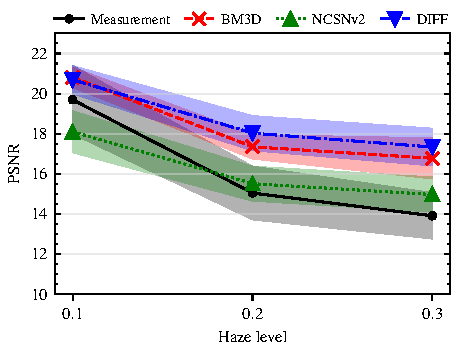
\includegraphics[trim=0 0.5em 0 0]{figures/steve9.pdf}
    \caption{Comparison of dehazing methods with harmonic imaging for varying levels of haze in the \emph{in-vitro} experiment. Shown are the average and standard deviation (shaded areas) of the PSNR over all frames. All pairs of PSNR scores pass the Welch’s t-Test for statistical significance ($p<0.05$), except for BM3D and DIFF at haze level $0.1$, and NCSNv2 and measurement at haze level $0.2$}
    \label{fig:haze_levels}
    \vspace{-0.5cm}
\end{figure}

\section{Results}
\color{black}

\subsection{In-Vitro}
\label{sec:res-invitro}
Fig.~\ref{fig:comparison-invitro} shows dehazing results on the phantom data. The RF-based diffusion dehazing method can reconstruct realistic dehazed images with improved contrast as well as provide plausible haze estimations. Both baseline methods (BM3D, NCSNv2) can remove most of the haze but at the cost of dropping signal from low-level tissue (typically endocardium). \color{black} This is often not acceptable in clinical practice as it hinders proper contouring of the left ventricle, in turn prohibiting accurate volume analysis or tracking for strain estimation. Lastly, we compare the proposed method against the baseline at various haze levels in Fig.~\ref{fig:haze_levels} and see an improved PSNR score across all haze levels.
\subsection{In-Vivo}
\color{black}
\label{sec:res-invivo}
The quantitative results on the dehazing of the \emph{in-vivo} are summarized in Fig.~\ref{fig:gcnr_subject} and \ref{fig:gcnr_view}, respectively. Fig.~\ref{fig:gcnr_subject} shows gCNR scores for both of the difficult-to-image subjects in the validation set, while Fig.~\ref{fig:gcnr_view} shows results for each of the four different acoustic windows. The spread in scores for each method can be mainly attributed to the variety of haze severity across sequences. Nonetheless, a clear pattern in the gCNR scores is detected. Compared to straightforward harmonic imaging, the BM3D method results in comparable and sometimes lower gCNR scores. This can be attributed to the excessive removal of signal by BM3D, which was also seen in the \emph{in-vitro} experiment. In contrast, the proposed diffusion method yields improved gCNR scores. Unlike the relatively good performance of the NCSNv2 supervised method on the phantom data, it fails to effectively remove the haze on the \emph{in-vivo} data, as expected for out-of-distribution data. Fig.~\ref{fig:ks-test} shows the KS test results on the \emph{in-vivo} dataset. Most notably, it can be seen that the proposed method retains speckle statistics in the myocardium region while altering the contents of the ventricle (read dehazing). Concerning the lateral resolution of the dehazing methods, the diffusion method strikes a balance between improving contrast, without sacrificing spatial resolution, see Fig.~\ref{fig:fwhm_lat_gcnr}. In comparison, the BM3D method compromises significantly on resolution, which is a common problem in denoising algorithms due to their smoothening nature.

A qualitative comparison is made in Fig.~\ref{fig:comparison-invivo}, where a representative set (bottom and top 10th percentile and mean gCNR scores) of the dehazed B-mode images is shown. A wider range of examples, including full cine-loops can be found on the online repository. From Fig.~\ref{fig:comparison-invivo} we observe that our diffusion method is more effective in removing haze compared to the supervised method. More importantly, apart from improved contrast, the proposed diffusion method retains and in some cases even reveals low-level tissue. Even though the \emph{in-vivo} data is out-of-distribution for the NCSNv2 model, the network can produce decent reconstructions due to the patch-based approach, showcasing the robustness of patch-based inference. Additionally, we show the posterior haze samples from the diffusion dehazing method, which resemble the haze samples used for training. We moreover observe that we can efficiently fine-tune the amount of dehazing by controlling the haze amplitude parameter $\gamma$ in the data-consistency step of our diffusion model. Note that this tunability is an inherent feature of the proposed reverse diffusion scheme with explicit data-consistency steps, and e.g. requires no gamma-specific training, in contrast to supervised methods, e.g. NCSNv2. Fig.~\ref{fig:varying_gamma} shows a comparison for varying $\gamma$-settings. The ability to fine-tune the algorithm's aggressiveness is highly beneficial, as optimal image quality is often subject to the personal preference of the user, which can significantly vary in clinical practice. Furthermore, sweeping the dehazing intensity allows the user to assess the quality of the output and set the optimal trade-off point with reduced haze and minimal signal loss, with the latter being crucial for diagnostic confidence. Automatic preference-based tuning of this parameter is an avenue for future work. Lastly, we assess the performance of the proposed diffusion method using a downstream delineation task as outlined in Section~\ref{sec:downstream} and observe that the diffusion-based processing aids EchoNet in producing more accurate delineations (Dice=0.891) compared to the hazy original image (Dice=0.880), as seen in Fig.~\ref{fig:echonet}. The Dice coefficients are averaged over the entire test set and computed with respect to the ground truth masks.

\begin{figure}
    \centering
    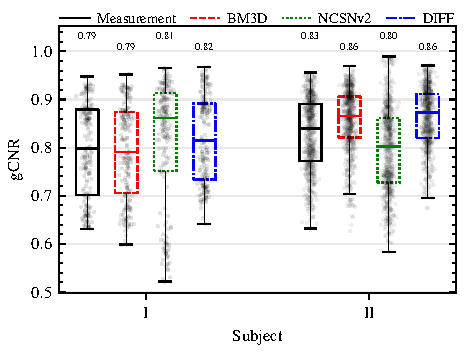
\includegraphics[trim=0 0 0 0.1cm]{figures/steve10.pdf}
    \caption{gCNR scores on the \emph{in-vivo} dataset grouped into separate subjects, comparing the raw harmonic images with baseline and proposed methods. Each dot represents a time frame within the acquisitions.}
    \label{fig:gcnr_subject}
\end{figure}
\begin{figure}
    \centering
    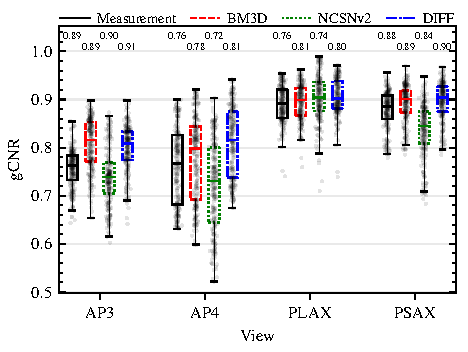
\includegraphics[trim=0 0 0 0.1cm]{figures/steve11.pdf}
    \caption{gCNR scores on the \emph{in-vivo} dataset grouped into the four different views, comparing the raw harmonic images with baseline and proposed methods. Each dot represents a time frame within the acquisitions.}
    \label{fig:gcnr_view}
    \vspace{-0.5cm}
\end{figure}
\begin{figure}
    \centering
    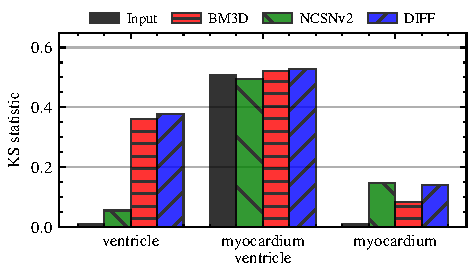
\includegraphics[trim=0 0.1cm 0 0]{figures/steve12.pdf}
    \caption{\TSW{Kolmogorov-Smirnov statistic for testing statistical similarity of the speckle in the myocardium and ventricle regions, pre- and post-dehazing. From left to right, we compare each of the two different regions of dehazing methods with the original data. The diffusion method retains the speckle statistics in the myocardium region, while clearly altering the contents from the ventricle. In contrast, the NCSNv2 method is not able to suppress haze in the ventricle area, leading to more similar statistics with respect to the input. As a reference, we also compare KS statistics between the dehazed ventricle and myocardium regions (middle column), which naturally are statistically different.}}
    \label{fig:ks-test}
\end{figure}
\begin{figure}
    \centering
    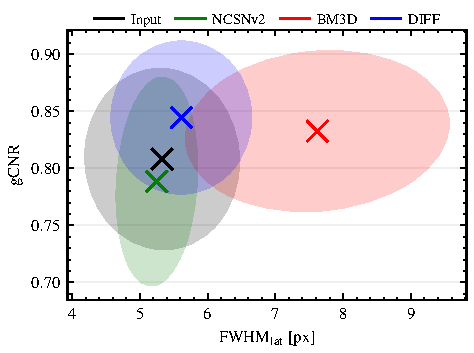
\includegraphics{figures/steve13.pdf}
    \caption{\TSW{Depiction of the FWHM of the myocardium speckle against the gCNR scores, depicting the inherent trade-off between contrast and lateral resolution. Each ellipse represents the average and standard deviation of each metric for that particular model. Our analysis reveals that the diffusion method both obtains high contrast and preserves lateral resolution, while the BM3D method compromises significantly on resolution.}}
    \label{fig:fwhm_lat_gcnr}
\end{figure}
\begin{figure*}
    \centering
    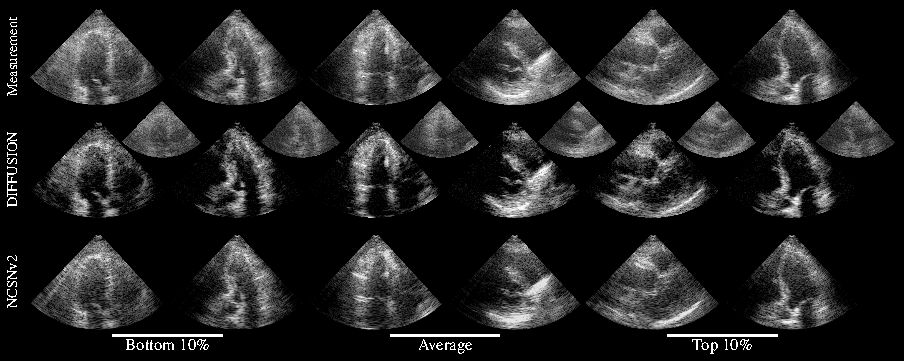
\includegraphics[width=\textwidth]{figures/steve14.pdf}
    \caption{\emph{In-vivo} results on a random selection of the validation dataset consisting of difficult-to-image subjects. \TSW{Before selection, images were sorted based on the gCNR score of the proposed diffusion method and divided into groups related to the bottom-10 and top-10 percentile and mean (within one standard deviation). We compare resulting B-mode images of the RF-based diffusion and supervised NCSNv2 dehazing methods.} The smaller inset plots show the haze posterior samples $\bh_0$ associated with each dehazed posterior ultrasound image $\bx_0$.}
    \label{fig:comparison-invivo}
\end{figure*}
\begin{figure}
    \centering
    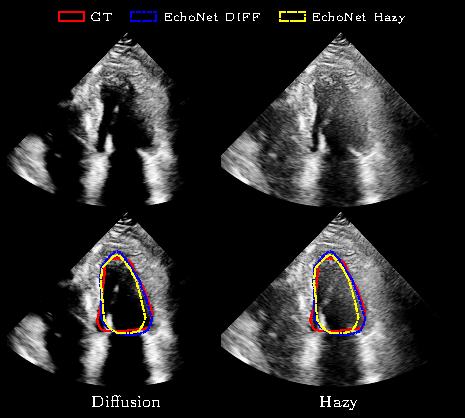
\includegraphics[width=\linewidth]{figures/steve15.pdf}
    \caption{\TSW{Downstream segmentation task with EchoNet on both hazy input from straightforward harmonic imaging, versus the diffusion-processed images. From the estimated masks, it can be seen that the hazy input data causes EchoNet to underestimate the ventricle area (yellow) with respect to the diffusion result (blue), which delineation is more in line with the ground truth (red).}}
    \label{fig:echonet}
    \vspace{-0.5cm}
\end{figure}